\chapter{Experiments and results}
\label{experiments_and_results}

\section{Experiments}
\label{experiments}

This section is devoted to explain the experiments performed using the algorithm presented in this thesis. It includes the implementation details, the experimental setup and the experiments themselves.

\subsection{Implementation details}
\label{experiments:implementation}
The software implementation has two main parts. The first one is in charge of communication with the sensor with the objective of extracting the depth data. This communication is performed using YARP\footnote{\url{http://www.yarp.it}}. YARP is a middleware software library \comment{(framework)} that leverages many common tasks required for a robot to work. Those tasks include actuator control and command, communications with the robot and between software parts, and accessing to different common sensors, such as depth sensors.

The second one is the implementation of the unfolding pipeline (algorithm). This implementation was executed using Python\footnote{\url{http://www.python.org}} as our language of choice. Python is a programming language that allows a quick development of prototype software, and that counts with a large collection of external libraries \comment{(modules)} to perform several tasks, from math calculations to computer vision. Our implementation is based on tho different computer vision libraries: OpenCV\footnote{\url{http://www.opencv.org}} and Scikit-image\footnote{\url{http://scikit-image.org}}, since during the development of this work several algorithms were evaluated. OpenCV is used for \comment{the basic vision stuff} and Scikit-image for more advanced algorithms such as Watershed \footnote{\url{http://scikit-image.org/docs/dev/auto_examples/plot_watershed.html}} and other superpixel-based clustering methods. Both libraries are compatible \comment{and working with both of them is not a problem}.

The whole unfolding algorithm implementation is Open Source, and is available online\footnote{\url{https://github.com/roboticslab-uc3m/textiles}}.

\subsection{Experimental Setup}
\label{experiments:expermimental_setup}

The algorithm was tested at our lab. The experimental setup consisted of several elements: a table, a depth sensor attached to a structure and a humanoid robot. The garment was placed on a white, flat surface, parallel to the floot. Over the garment, an ASUS Xtion PRO LIVE depth sensor was placed to capture data from a top view. The unfolding operation is performed by a 

\comment{[...]}

The starting point for testing our algorithm is the data adquisition process. Data is obtained as a point cloud from a ASUS Xtion Pro Live sensor. Then, it is converted to a depth map image for its later analysis. 

This conversion is done by simply using the z component of each point as the depth value for each pixel of the depth image. This depth image could also be recovered from the point cloud using the instrinsic and extrinsic parameters of the sensor. But, as the sensor is placed on top of the garment, perpendicular to the surface on which the clothing article rests, both methods yield almost very similar results.

\begin{figure}[thpb]
    \centering
    
\includegraphics[width=0.7
    \textwidth]{figures/placeholder2.png}
    \caption{\comment{Here I should put a nice figure of the point cloud and the depth image}}
    \label{fig:point_cloud_and_depth_image}
\end{figure}

The RGB values are also recorded for each depth image, obtaining an RGB-D image.

\subsection{Experiments \comment{(Other stuff)}}
\label{experiments:experiments}

The final experiments using the current algorithm have been performed using an ASUS Xtion PRO LIVE at 640x480 RGB and depth streams (30 fps).
To simplify the image analysis, the sensor is placed on top of the working surface  providing a bird's eye view over the cloth folding environment, with its image plane almost parallel to the working surface.

In the present work we are using thick blankets and towels, to cope with the limitations of the resolution of the depth sensor. A set of six samples with one or two folds were presented to the system for analysis. The results are shown in Fig. \ref{directions}.
%
These results show that the algorithm generates acceptable unfolding directions.

%However, when analyzing the experimental results, one can see that the candidate paths for unfolding are created using the garment contour segment midpoint. This fact can warp the most intuitive direction, which would be the closest between the highest region and the garment contour.

According to the results, an interpolation between the best two directions could result in a better solution. The best directions for the set of clothes are shown in Fig. \ref{directions_several}. %The arrow's directions make us believe that a combined directions by averaging them could provide better results.

%\warning{In \cite{Li2015IROS}, Li et al. present a method for folding deformable objects such as clothes. }

%A final demonstration of the current algorithm has been performed using the full-size humanoid robot TEO \cite{martinez2012teo}. Depth sensor coordinates are passed to the robot root frame, and a standard pick and place operation is performed with the given points. Figure \ref{setup} depicts this scenario.

\section{Data adquisition}
\label{data_adquisition}

The starting point of our algorithm is the data adquisition process. Data is obtained as a point cloud from a ASUS Xtion Live sensor. Then, data is converted to a depth map image for its later analysis. 

This conversion is done by simply using the z component of each point as the depth value for each pixel of the depth image. This depth image could also be recovered from the point cloud using the instrinsic and extrinsic paramters of the sensor. But, as the sensor is placed on top of the garment, perpendicular to the surface on which the clothing article rests, both methods yield almost very similar results.

\begin{figure}[thpb]
    \centering
    
\includegraphics[width=0.7
    \textwidth]{figures/placeholder2.png}
    \caption{\comment{Here I should put a nice figure of the point cloud and the depth image}}
    \label{fig:point_cloud_and_depth_image}
\end{figure}

The RGB values are also recorded for each depth image, obtaining an RBG-D image.

\section{Results}
\label{results}

\begin{figure}[thpb]
    \centering
    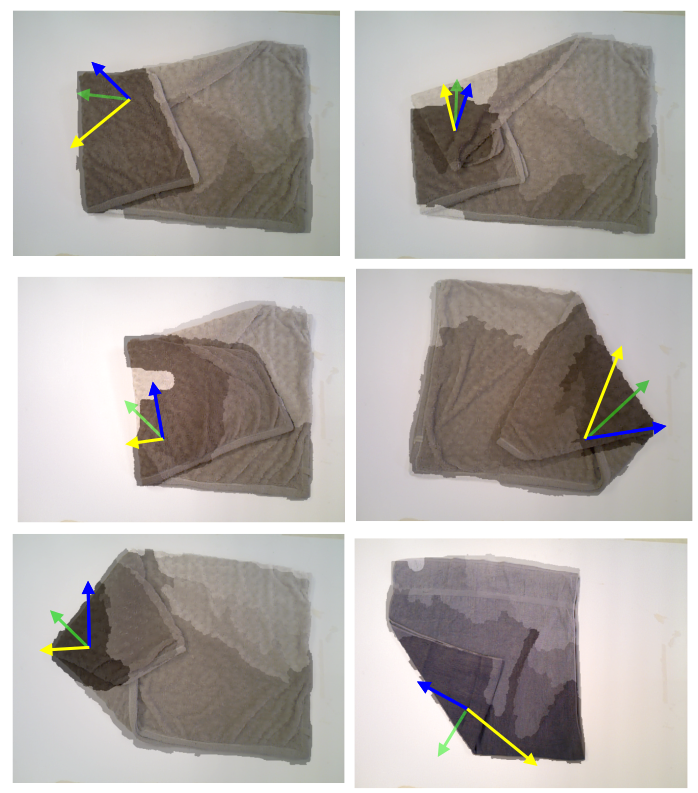
\includegraphics[width=0.48\textwidth]{figures/directions_several.png}
    \caption{Best directions calculated for each garment provided to the system. The direction with the smallest bumpiness value is shown in blue. The second best direction is shown in yellow. The bisector is shown in green. The arrows are for demonstrative purpose only, and their starting and ending point do not represent the pick and place point. The watershed computed regions are additionally overlaid upon the original image.}
    \label{directions_several}
\end{figure}
